\documentclass{beamer}

% Font selection
\usepackage{palatino}

% Beamer template
\usetheme{Antibes}
%\usetheme{Berlin}

\usepackage[scale=1.2]{ccicons}

\usepackage[utf8]{inputenc}
\usepackage[T1]{fontenc}

\usepackage{tabularx}
\usepackage{multicol}
\usepackage{graphicx}
\usepackage[final]{pdfpages}

\usepackage{listings}

\lstset{
  language=[ISO]C++,
  columns=flexible,
  identifierstyle=\itshape,
%
  belowcaptionskip=1\baselineskip,
  breaklines=true,
  xleftmargin=\parindent,
  language=C++,
  showstringspaces=false,
  basicstyle=\small,
  keywordstyle=\bfseries\color{green!40!black},
  commentstyle=\itshape\color{purple!40!black},
  identifierstyle=\color{blue},
  stringstyle=\color{brown},
  columns=flexible,
%  inputenconding=utf8,
  extendedchars=true,
%
  morekeywords=[1]{constexpr,nullptr,alignof,alignas,decltype,noexcept,override,final,concept,expects,ensures,assert},
  literate={%
    {¿}{{?`}}1
    {¡}{{!`}}1
    {á}{{\'a}}1
    {é}{{\'e}}1
    {í}{{\'i}}1
    {ó}{{\'o}}1
    {ú}{{\'u}}1
    {ñ}{{\~n}}1
}
}

\lstset{
}


\newcommand{\cppkey}[1]{%
{\color{green!40!black}\textbf{#1}}%
}

\newcommand{\cppid}[1]{%
{\color{blue}\textbf{#1}}%
}


\usepackage{tikz}
\usetikzlibrary{positioning}
\usetikzlibrary{arrows}
\usetikzlibrary{mindmap}

\usepackage{pgfplots}
\pgfplotsset{compat=1.5}


\newcommand{\textgood}[1]{%
{\color{blue}\textbf{#1}}%
}

\newcommand{\textbad}[1]{%
{\color{red}\textbf{#1}}%
}

\newcommand{\textenum}[1]{%
{\color{blue!60!black}\textbf{#1}}%
}

\newcommand{\textmark}[1]{%
{\color{orange!70!black}\textbf{#1}}%
}




% Footline in every slide
\setbeamertemplate{footline}{
  \leavevmode%
  \hbox{\begin{beamercolorbox}[wd=\paperwidth,ht=2.5ex,dp=1.125ex,leftskip=.3cm,rightskip=.3cm]{author in head/foot}%
    \usebeamerfont{author in head/foot}\ccbyncndeu 
     \quad -- \quad J. Daniel Garcia 
     -- ARCOS@UC3M (\textbf{\url{josedaniel.garcia@uc3m.es}}) 
     -- Twitter: \textbf{\url{@jdgarciauc3m}}
    \hfill
    \insertframenumber/\inserttotalframenumber
  \end{beamercolorbox}}%
  \vskip0pt%
}

% Logo in every slide
\addtobeamertemplate{headline}{}
{% 
\begin{tikzpicture}[remember picture,overlay]
\node[anchor=north east] at (current page.north east) {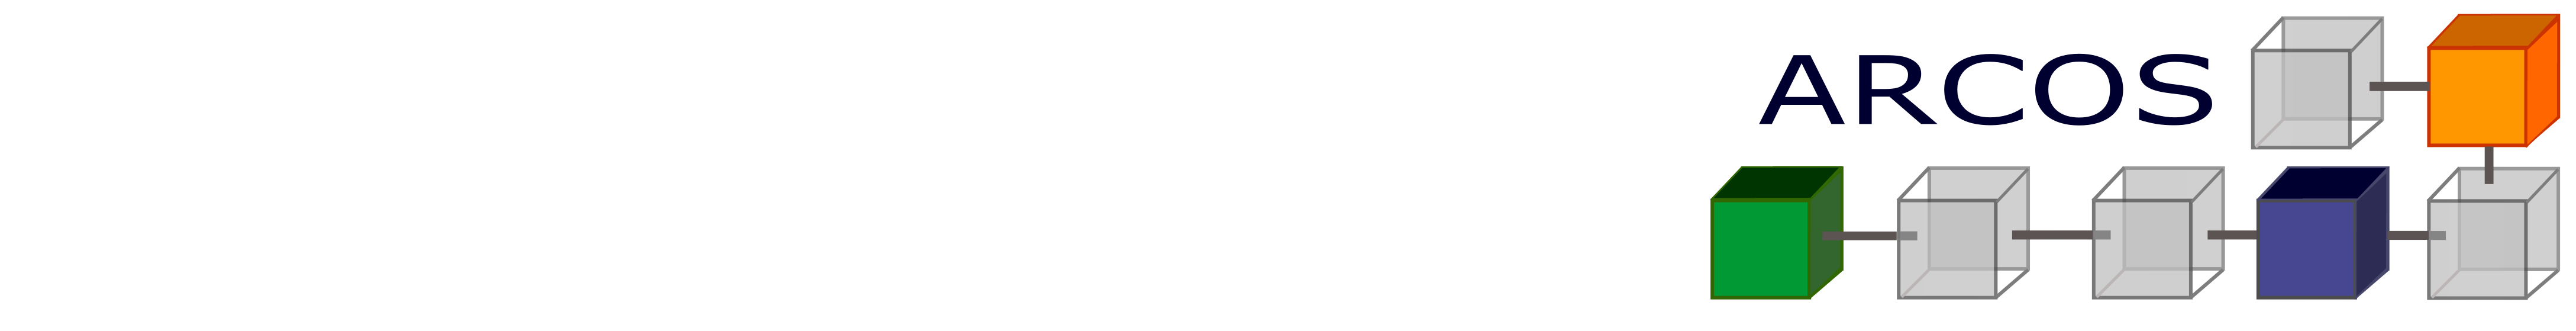
\includegraphics[height=0.7cm]{logos/arcos_t.png}};
\end{tikzpicture}
}

\tikzset{
  invisible/.style={opacity=0},
  visible on/.style={alt=#1{}{invisible}},
  alt/.code args={<#1>#2#3}{%
    \alt<#1>{\pgfkeysalso{#2}}{\pgfkeysalso{#3}} % \pgfkeysalso doesn't change the path
  },
}

%Portada
\title{Parallelism support in C++17}
\subtitle{A library solution}
\author{J. Daniel Garcia}
\institute{ARCOS Group\\University Carlos III of Madrid\\Spain}
\date{January, 23th 2018}

\begin{document}

\begin{frame}
\titlepage
\end{frame}

\AtBeginSection[]
{
  \begin{frame}<*>
    \setbeamertemplate{section in toc shaded}[default][50]
    \setbeamertemplate{subsection in toc shaded}[default][50]
    \tableofcontents[currentsection,hideallsubsections]
  \end{frame}
}

\AtBeginSubsection[]
{
  \begin{frame}<beamer>
    \setbeamertemplate{subsection in toc shaded}[default][50]
    \tableofcontents[sectionstyle=show/hide,subsectionstyle=show/shaded/hide]
  \end{frame}
}

\begin{frame}{Warning}

\begin{tabularx}{.98\textwidth}{lX}
\ccLogo & This work is under 
Attribution-NonCommercial-NoDerivatives 4.0 International (CC BY-NC-ND 4.0) license.\\

& You are \textbf{free} to
\textbf{Share} — copy and redistribute the material in any medium or format.
\\

\ccAttribution & 
You must give appropriate credit, provide a link to the license, and indicate if changes were made. You may do so in any reasonable manner, but not in any way that suggests the licensor endorses you or your use.\\

\ccNonCommercialEU &
You may not use the material for commercial purposes.
\\

\ccNoDerivatives &
If you remix, transform, or build upon the material, you may not distribute the modified material.
\\

\end{tabularx}

\end{frame}

\begin{frame}{ARCOS@uc3m}
\begin{itemize}
  \item \textbf{UC3M}: A young international research oriented university.
  \vfill
  \item \textbf{ARCOS}: An applied research group.
    \begin{itemize}
      \item {\color{blue}{Lines}}: 
            High Performance Computing,
            Big data,
            Cyberphysical systems,
            \alert{Programming Models for Applications Improvement}.
    \end{itemize} 
  \vfill
  \item \textbf{Improving applications}:
    \begin{itemize}
      \item \textbf{REPARA}: Reengineering and Enabling Performance and poweR of Applications.
            (FP7).
      \item \textbf{RePhrase}: REfactoring Parallel Heterogeneous Resource Aware Applications.
            (H2020).
    \end{itemize} 
  \vfill
  \item \textbf{Standardization}:
    \begin{itemize}
      \item ISO/IEC JTC/SC22/WG21. Comité ISO C++.
    \end{itemize}
\end{itemize}
\end{frame}

\section{C++17 is here}
\begin{frame}[t]{C++: An evolving language}
\begin{center}
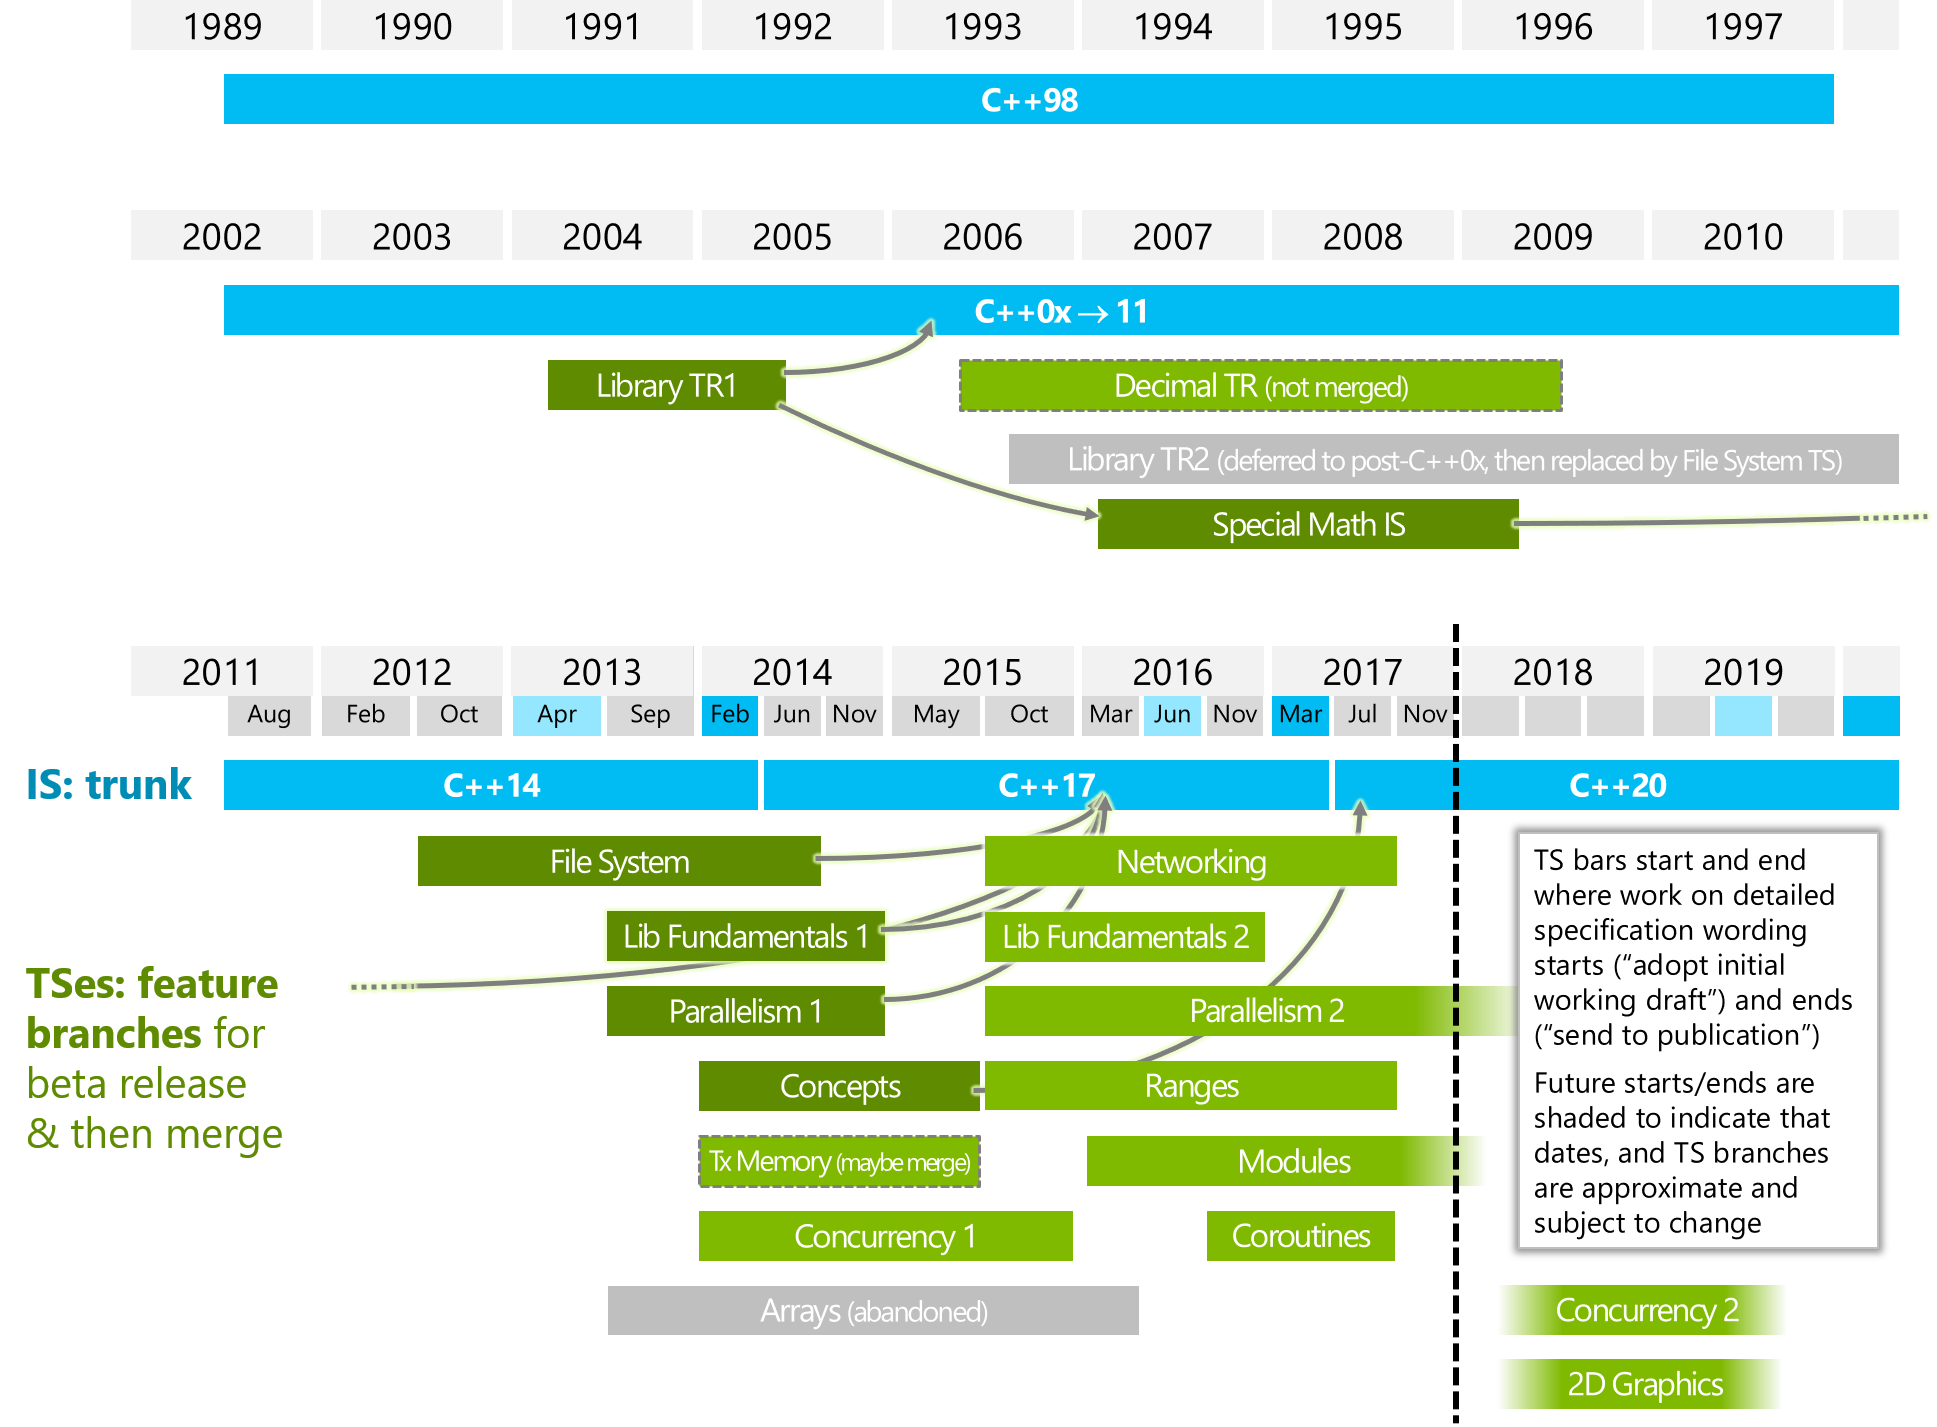
\includegraphics[height=.85\textheight]{img/wg21-timeline.png}
\end{center}
\end{frame}

\begin{frame}[t]{From C++98 to C++11}
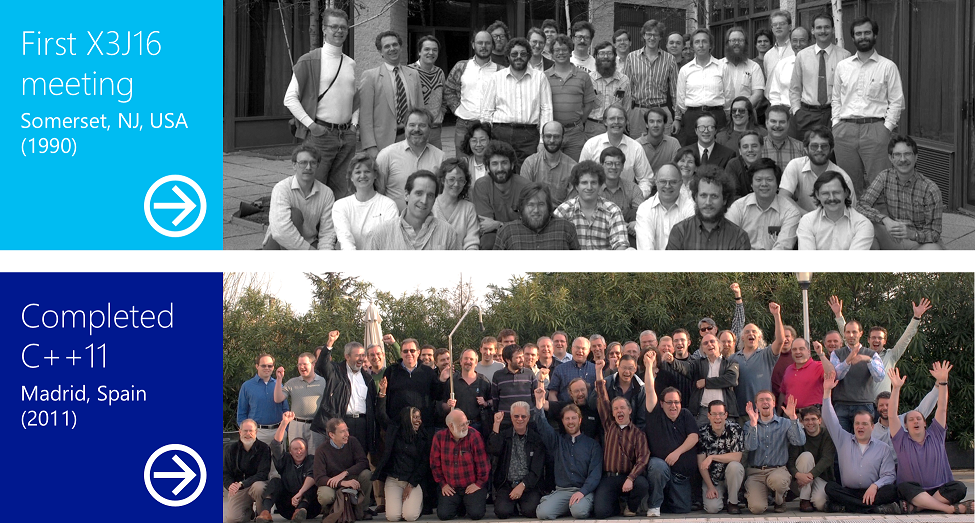
\includegraphics[width=\textwidth]{img/wg21-1990-2011.png}
\end{frame}

\begin{frame}[t]{C++14}
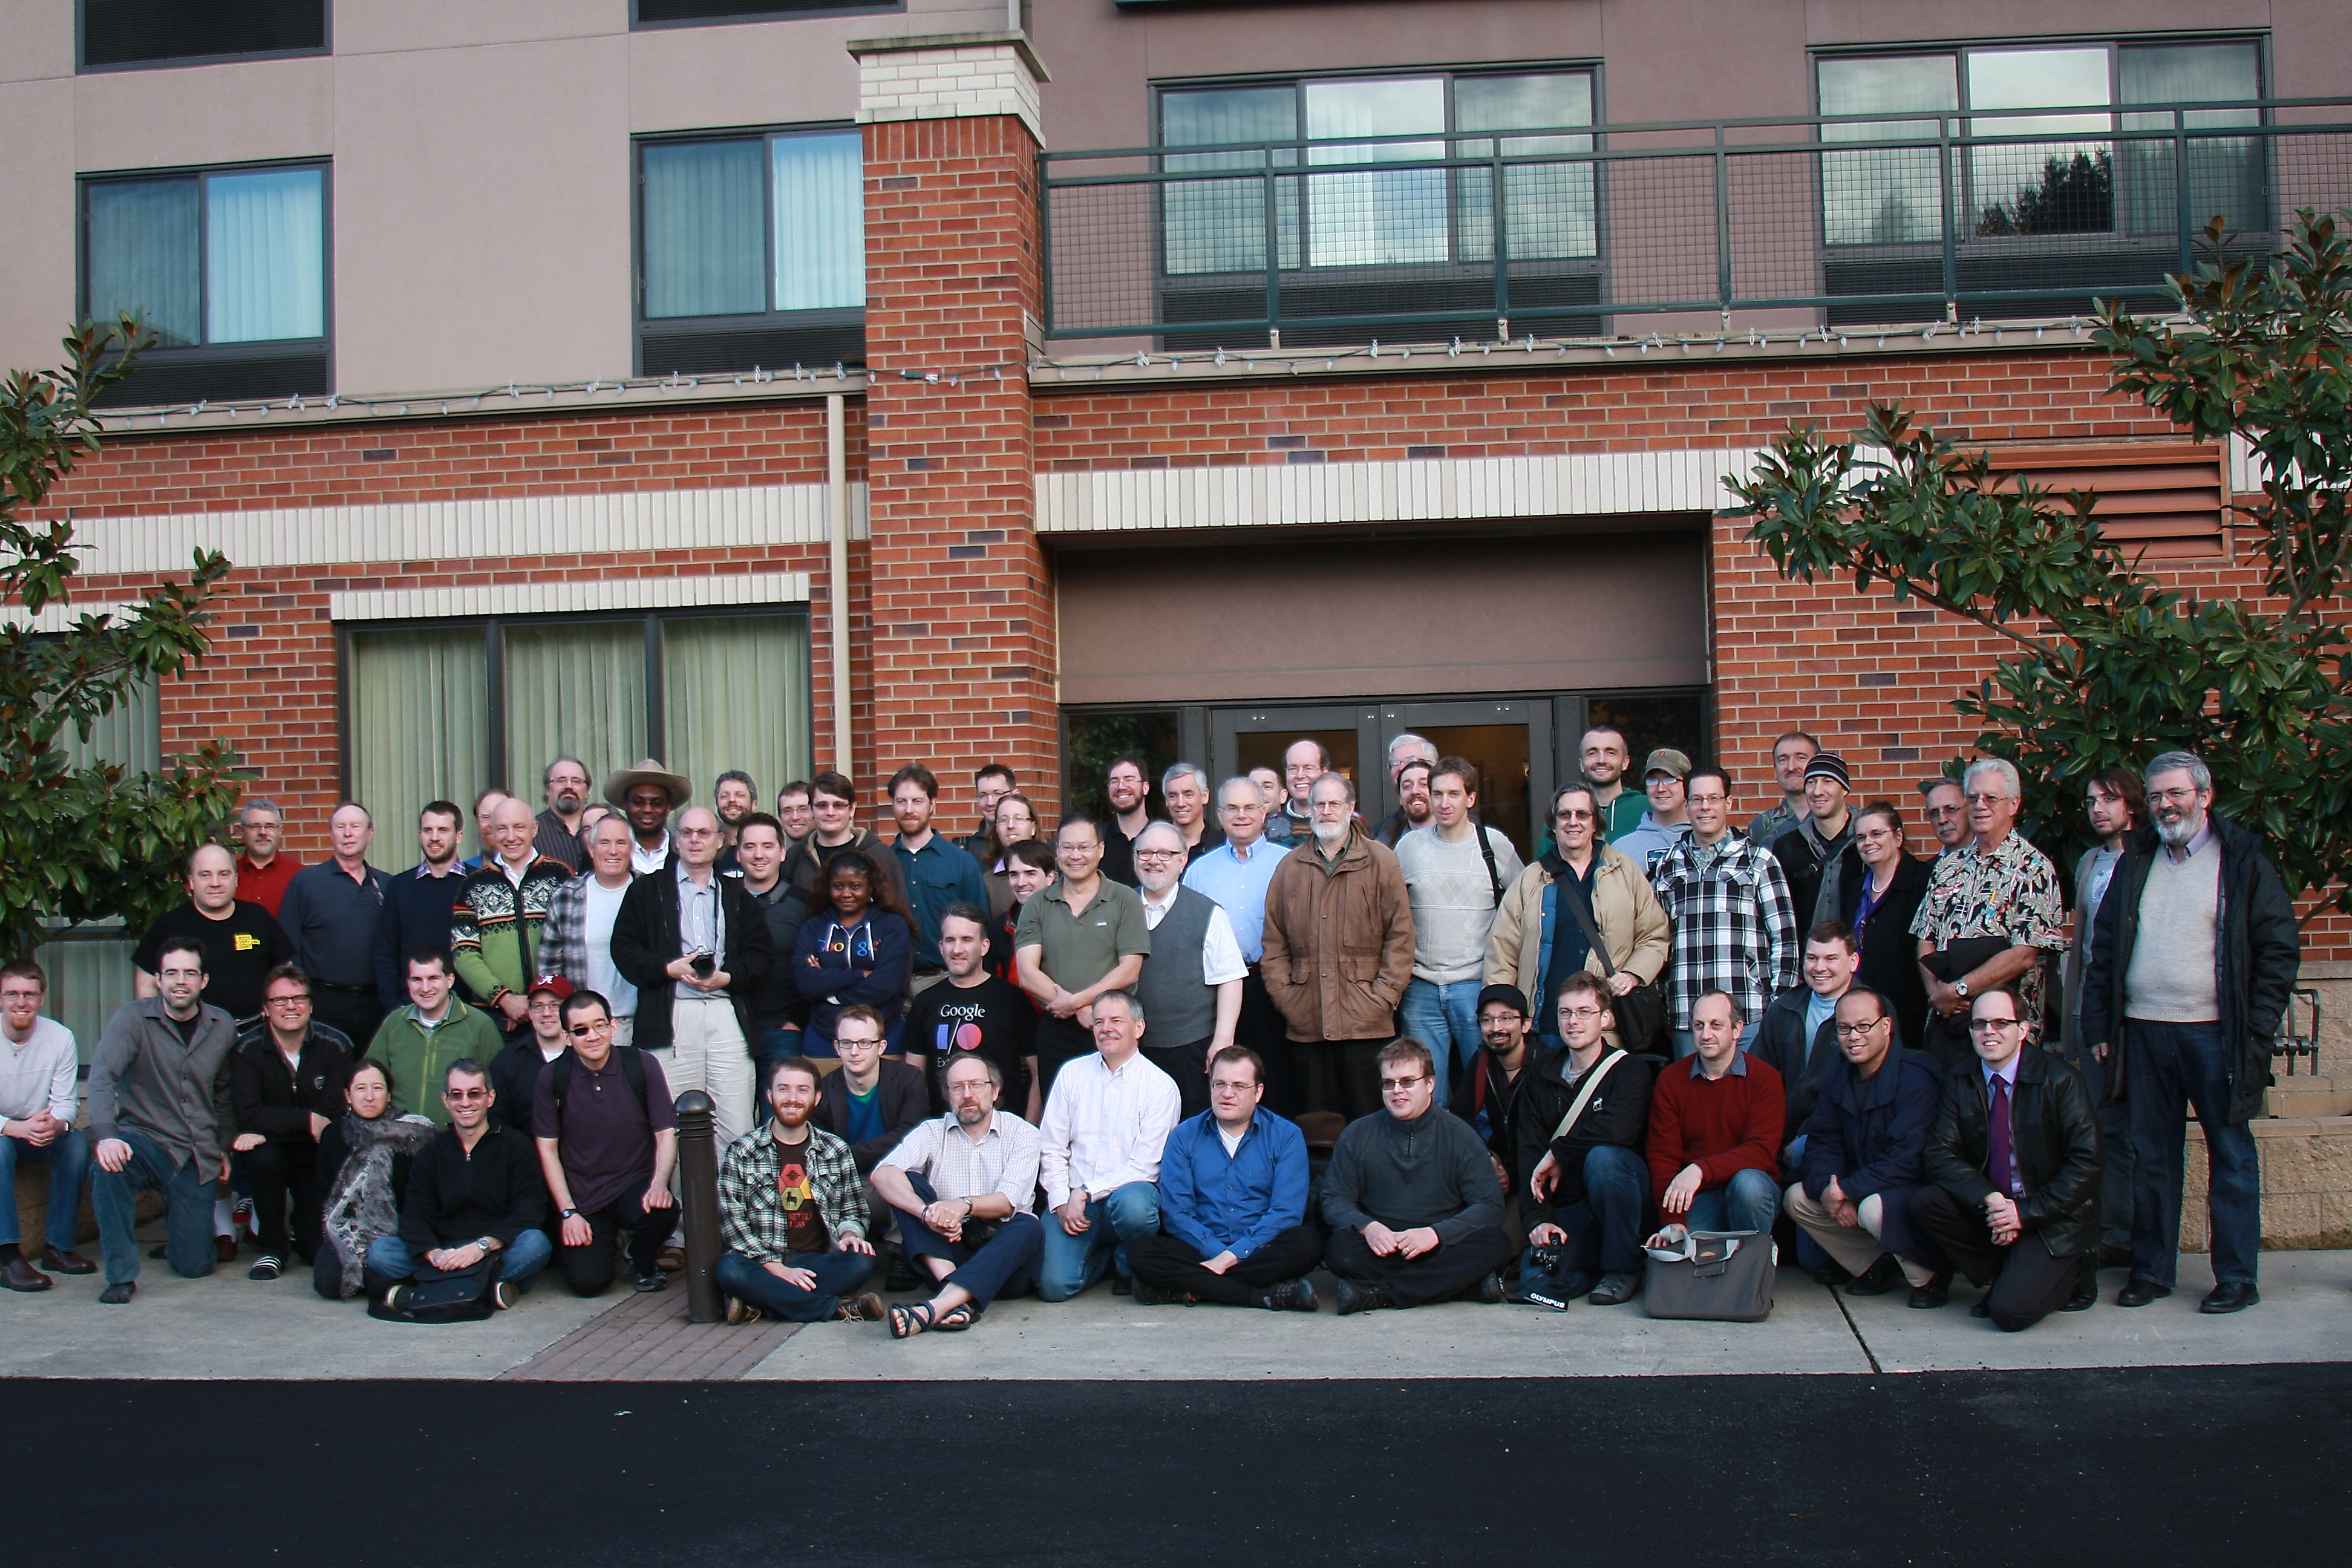
\includegraphics[width=\textwidth]{img/cpp-14.jpg}
\end{frame}

\begin{frame}[t]{C++17}
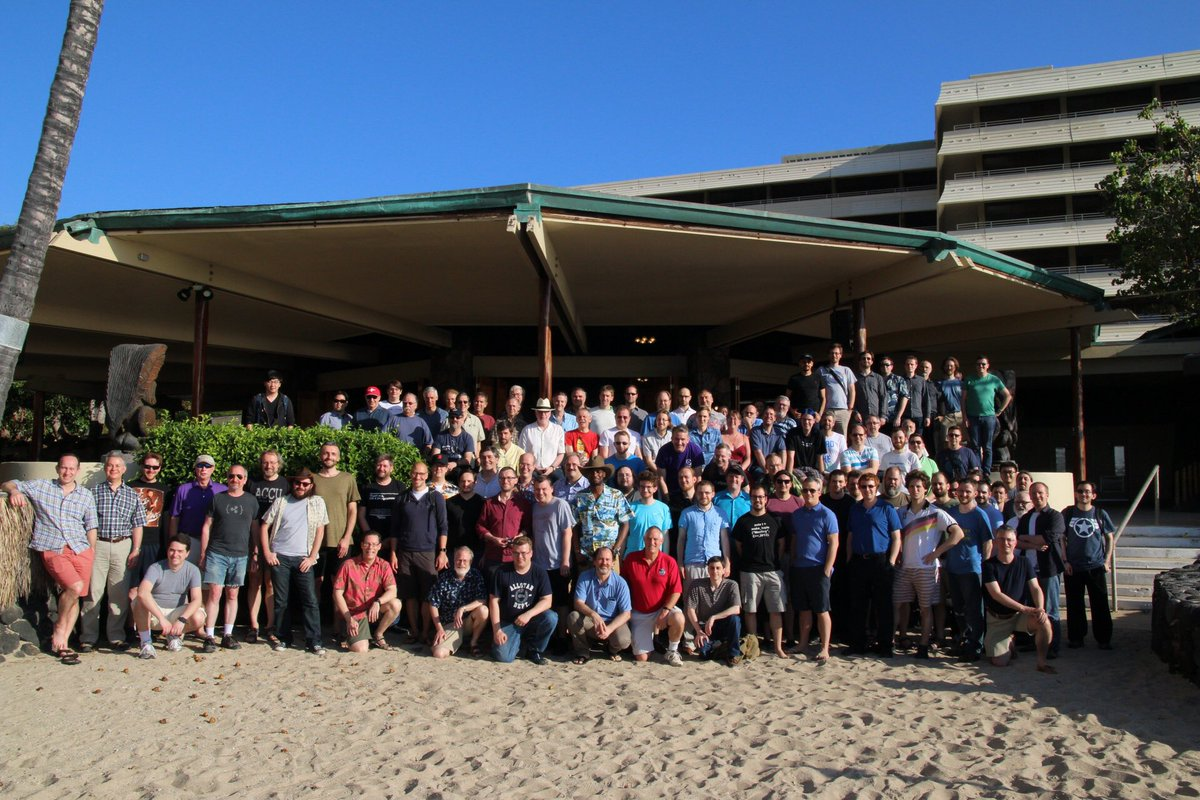
\includegraphics[width=\textwidth]{img/cpp-17.jpg}
\end{frame}

\begin{frame}[t]{What's new?}
\begin{itemize}
  \item Removing old stuff (e.g. trigraphs, \cppkey{register}, \cppid{auto\_ptr}, \ldots).
  \vfill\pause
  \item Clarifications (order of evaluation, copy elision, \ldots).
  \vfill\pause
  \item Better support for generic programming.
    \begin{itemize}
      \item Template argument deduction for classes.
      \item Expression folding.
      \item Compile time \cppkey{if}.
    \end{itemize}
  \vfill\pause
  \item Language simplifications:
    \begin{itemize}
      \item Structured binding.
      \item Initialization in \cppkey{if}/\cppkey{switch}.
    \end{itemize}
  \vfill\pause
  \item Library enhancements:
    \begin{itemize}
      \item \cppid{any}, \cppid{optional}, \cppid{variant}, \cppid{string\_view}.
      \item \cppid{filesystem}.
    \end{itemize}
  \vfill\pause
  \item \textbad{Parallel algorithms library}.
\end{itemize}
\end{frame}


\section{Execution policies in C++17}
\begin{frame}[t]{Policies}
\begin{itemize}
  \item An \textgood{execution policy}
        selects the kind of parallelism to run an algorithm.
    \begin{itemize}

      \vfill\pause
      \item \textmark{Sequential}: No parallelism.
        \begin{itemize}
          \item Type : \cppid{std::execution::sequenced\_policy}
          \item Global object: \cppid{std::execution::seq}.
        \end{itemize}

      \vfill\pause
      \item \textmark{Parallel}: Parallelized.
        \begin{itemize}
          \item Type : \cppid{std::execution::parallel\_policy}.
          \item Global object: \cppid{std::execution::par}.
        \end{itemize}

      \vfill\pause
      \item \textmark{Parallel + Vector}: Parallelized and vectorized.
        \begin{itemize}
          \item Type: \cppid{std::execution::parallel\_unsequenced\_policy}.
          \item Global object: \cppid{std::execution::par\_unseq}.
        \end{itemize}
    \end{itemize}
\end{itemize}
\end{frame}

\begin{frame}[t,fragile]{Algorithms versions}
\begin{itemize}
  \item All algorithm versions take as first argument an execution policy.
\end{itemize}
\begin{block}{Example: sorting a vector}
\begin{lstlisting}[]
using namespace std;
vector<double> v = read_values();
sort(v.begin(), v.end());

using namespace std::execution;

sort(seq, v.begin(), v.end()); // Sequential
sort(par, v.begin(), v.end()); // Parallel
sort(par_unseq, v.begin(), v.end()); // Par + Vector
\end{lstlisting}
\end{block}
\end{frame}



\section{General overview of algorithms}
\begin{frame}[t]{Which algorithms ar included?}
\begin{itemize}
  \item Most STL algorithm include now a parallel version.
  \item A new argument signals the execution policy.
    \begin{itemize}
      \item The execution is the first argument.
    \end{itemize}
  \item Some algorithms do not have a parallel counterpart.
    \begin{itemize}
      \item Example: \cppid{accumulate}.
    \end{itemize}
  \item Some new algorithms not coming from the STL.
    \begin{itemize}
      \item Example: \cppid{exclusive\_scan}
    \end{itemize}
\end{itemize}
\end{frame}

\begin{frame}[t,allowframebreaks]{Operaciones invariantes sobre secuencias}
\begin{itemize}
  \item \textmark{Iteration}: 
    \cppid{for\_each}, 
    \cppid{for\_each\_n}.

  \vfill
  \item \textmark{Counting}: 
    \cppid{count}, 
    \cppid{count\_if}.

  \vfill
  \item \textmark{Finding values}: 
    \cppid{adjacent\_find}, 
    \cppid{find}, 
    \cppid{find\_if},
    \cppid{find\_if\_not}.

  \vfill
  \item \textmark{Searching subsequences}:
    \cppid{search},
    \cppid{search\_n}.

  \vfill
  \item \textmark{Sequence comparison}: 
    \cppid{equal},
    \cppid{mismatch}.

  \vfill
  \item \textmark{Predicate checking}: 
    \cppid{all\_of}, 
    \cppid{any\_of},
    \cppid{none\_of}.
\end{itemize}
\end{frame}

\begin{frame}[t,fragile]{Finding in a sequence}
\begin{block}{Examples}
\begin{lstlisting}[]
vector<int> v = get_values_vector();

// Count positive values
count_if(par, begin(v), end(v), 
  [](int x) { return x>0; });

// Find first value equal to 0
auto p = find(par, begin(v), end(v), 0);

// Find first value greater than 0 and less than 10
auto q = find_if(par, begin(v), end(v),
  [](int x) { return (x>0) && (x<10); }
\end{lstlisting}
\end{block}
\end{frame}

\begin{frame}[t,allowframebreaks]{Modifying sequence operations}
\begin{itemize}
  \item \textmark{Copying}:
    \cppid{copy},
    \cppid{copy\_if},
    \cppid{copy\_n}
  \item \textmark{Moving}:
    \cppid{move}.
  \item \textmark{Populating a sequence}:
    \cppid{fill},
    \cppid{fill\_n},
    \cppid{generate},
    \cppid{generate\_n}.
  \item \textmark{Element removal}:
    \cppid{remove},
    \cppid{remove\_if},
    \cppid{remove\_copy},
    \cppid{remove\_copy\_if}.
  \item \textmark{Replacement}:
    \cppid{replace},
    \cppid{replace\_if},
    \cppid{replace\_copy},
    \cppid{replace\_copy\_if},
    \cppid{unique},
    \cppid{unique\_copy}.
  \item \textmark{Element reordering}:
    \cppid{reverse},
    \cppid{reverse\_copy},
    \cppid{rotate},
    \cppid{rotate\_copy}.
  \item \textmark{Swaping}: \cppid{swap\_ranges}.
  \item \textmark{Element transformation}: \cppid{transform}.
\end{itemize}
\end{frame}

\begin{frame}[t,allowframebreaks]{Partitioning, sorting and set}
\begin{itemize}
  \item \textmark{Partitioning}:
    \cppid{is\_partitioned},
    \cppid{partition},
    \cppid{partition\_copy},
    \cppid{stable\_partition}.
  \item \textmark{Sorting}:
    \cppid{partial\_sort},
    \cppid{partial\_sort\_copy},
    \cppid{sort},
    \cppid{stable\_sort}.
  \item \textmark{Auxiliary to sorting}:
    \cppid{is\_sorted},
    \cppid{is\_sorted\_until},
    \cppid{nth\_element}.
  \item \textmark{Heap operations}:
    \cppid{is\_heap},
    \cppid{is\_heap\_until}.
  \item \textmark{Set operations}:
    \cppid{includes},
    \cppid{inplace\_merge},
    \cppid{merge},
    \cppid{set\_difference},
    \cppid{set\_intersection},
    \cppid{set\_symmetric\_difference},
    \cppid{set\_union}.
\end{itemize}
\end{frame}

\begin{frame}[t]{Other}
\begin{itemize}
  \item \textmark{Min and max}:
    \cppid{lexicographical\_compare},
    \cppid{max\_element},
    \cppid{min\_element},
    \cppid{minmax\_element}.
  \item \textmark{Memory operations}:
    \cppid{uninitialized\_copy},
    \cppid{uninitialized\_copy\_n},
    \cppid{uninitialized\_fill},
    \cppid{uninitialized\_fill\_n}.
\end{itemize}
\end{frame}

  
\begin{frame}[t]{Numerics}
\begin{itemize}
  \item \textmark{Reduction}:
    \cppid{reduce},
    \cppid{transform\_reduce}.
  \item \textmark{Scans}:
    \cppid{exclusive\_scan},
    \cppid{inclusive\_scan},
    \cppid{transform\_exclusive\_scan},
    \cppid{transform\_inclusive\_scan}.
  \item \textmark{Others}:
    \cppid{adjacent\_difference}.
\end{itemize}
\end{frame}



\section{Non-numeric algorithms}
\begin{frame}[t]{Non-numeric algorithms}
\begin{itemize}
  \item Do not require value that value type is a numeric type.
    \begin{itemize}
      \item More general than numeric types.
    \end{itemize}

  \vfill
  \item Examples:
    \begin{itemize}
      \item \cppid{for\_each()}.
      \item \cppid{for\_each\_n()}.
    \end{itemize}

  \vfill
  \item Might be considered equivalent to a \textmark{parallel-for}.
\end{itemize}
\end{frame}

\begin{frame}[t,fragile]{For Each}
\begin{lstlisting}[]
template <class ExecutionPolicy, class InputIterator, 
          class Function>
void for_each(ExecutionPolicy && ep, 
              InputIterator first, InputIterator last, Function f);
\end{lstlisting}
\begin{itemize}
  \item Applies \cppid{f} to every value in range \cppid{[first,last)}.
\end{itemize}
\begin{block}{Example}
\begin{lstlisting}[basicstyle=\scriptsize]
long count_primes(const vector<int> & v) {
  std::atomic<long> count;
  for_each(par, begin(v), end(v), [&](int x) {
    if (is_prime(x)) { count++; }
  });
  return count;
}
\end{lstlisting}
\end{block}
\end{frame}

\begin{frame}[t,fragile]{For Each}
\begin{lstlisting}[]
template <class ExecutionPolicy, class InputIterator, 
          class Size, class Function>
void for_each_n(ExecutionPolicy && ep, 
                InputIterator first, Size n, Function f);
\end{lstlisting}
\begin{itemize}
  \item Applies \cppid{f} to every value in range \cppid{[first,first+n)}.
\end{itemize}
\begin{block}{Example}
\begin{lstlisting}[basicstyle=\scriptsize]
long count_primes(const vector<int> & v, int k) {
  std::atomic<long> count;
  for_each_n(par, begin(v), k, [&](int x) {
    if (is_prime(x)) { count++; }
  });
  return count;
}
\end{lstlisting}
\end{block}
\end{frame}

\begin{frame}[t,fragile]{But...}
\begin{itemize}
  \item \cppid{for\_each} is not usually the best way to do things.
\end{itemize}
\begin{block}{Example}
\begin{lstlisting}[basicstyle=\scriptsize]
long count_primes(const vector<int> & v) {
  return count_if(par, begin(v), end(v), [&](int x) {
    return is_prime(x);
  });
}
\end{lstlisting}
\end{block}
\end{frame}


\section{Numeric algorithms: reduce and scan}
\begin{frame}[t]{Numeric algorithm}
\begin{itemize}
  \item Algorithms for \textgood{numeric sequences}.
    \begin{itemize}
      \item \textmark{Reduction}:
        \begin{itemize}
          \item \cppid{reduce}.
          \item \cppid{transform\_reduce}.
        \end{itemize}
      \item \textmark{Scan}:
        \begin{itemize}
          \item \cppid{exclusive\_scan}.
          \item \cppid{inclusive\_scan}.
          \item \cppid{transform\_exclusive\_scan}.
          \item \cppid{transform\_inclusive\_scan}.
        \end{itemize}
    \end{itemize}
  \vfill
  \item Also sequential versions without execution policy.
\end{itemize}
\end{frame}

\begin{frame}[t]{GENERALIZED\_SUM}
\begin{itemize}
  \item Building block for defining reductions.
  \vfill
  \item \cppid{GENERALIZED\_SUM(op, a$_1$, \ldots, a$_n$)}:
    \begin{itemize}
      \item \cppid{op(GENERALIZED\_SUM(op,b$_1$,\ldots, b$_k$), GENERALIZED\_SUM(op,b$_l$, \ldots, b$_n$))}.
      \item \cppid{b$_1$, \ldots, b$_k$,b$_l$, \ldots, b$_n$} is a permutation of \cppid{a$_1$, \ldots, a$_n$}.
    \end{itemize}
  \vfill
  \item \textmark{Impact}:
    \begin{itemize}
      \item Subranges may be grouped and rearranged.
      \item Assumes \cppid{op} is commutative.
    \end{itemize}
\end{itemize}
\end{frame}

\begin{frame}[t,fragile]{reduce}
\begin{lstlisting}[]
template <class ExecutionPolicy, class ForwardIterator, class T, class BinaryOperation>
T reduce(ExecutionPolicy && policy, ForwardIterator first, ForwardIterator last, T init, BinaryOperation op);
\end{lstlisting}
\begin{itemize}
  \item \cppid{GENERALIZED\_SUM(op, init, *first, \ldots )}
  \item \cppid{op} Cannot \textbad{invalidate} the iterators.
  \item \cppid{op} Cannot \textbad{modify} values in the range.
  \item \cppid{reduce} might be \textbad{non-deterministic} when \cppid{op} es non associative or non-commutative.
\end{itemize}
\begin{block}{Example: Adding values in a vector}
\begin{lstlisting}[]
sum = reduce(par, begin(v), end(v), 0, [](int a, int b) { 
  return a+b; });
\end{lstlisting}
\end{block}
\end{frame}

\begin{frame}[t,fragile]{Defaulting operation in reduce}
\begin{lstlisting}[]
template <class ExecutionPolicy, class InputIterator, class T, class BinaryOperation>
T reduce(ExecutionPolicy && policy, InputIterator first, InputIterator last, T init);
\end{lstlisting}
\begin{itemize}
  \item Defaults to addition.
  \item \cppid{reduce(first,last,init,plus<>())}.
\end{itemize}
\vfill
\begin{block}{Example: Adding values in a vector}
\begin{lstlisting}[]
sum = reduce(par, begin(v), end(v), 0);
\end{lstlisting}
\end{block}
\end{frame}

\begin{frame}[t,fragile]{Defaulting operation and initial value in reduce}
\begin{lstlisting}[]
template <class ExecutionPolicy, class InputIterator>
T reduce(ExecutionPolicy && policy, InputIterator first, InputIterator last);
\end{lstlisting}
\begin{itemize}
  \item Defaults to addition.
  \item Defaults initial value to value type default value.
  \item \cppid{reduce(first, last, iterator\_traits<ForwardIt>::value\_type\{\}, plus<>())}.
\end{itemize}
\vfill
\begin{block}{Example: Adding values in a vector}
\begin{lstlisting}[]
sum = reduce(par, begin(v), end(v));
\end{lstlisting}
\end{block}
\end{frame}

\begin{frame}[t,fragile]{Transform reduce}
\begin{lstlisting}[]
template <class ExecutionPolicy, class InputIterator, class T, class UnaryOp, class BinaryOp>
T transform_reduce(ExecutionPolicy && policy, InputIterator first, InputIterator last, UnaryOp unary_op, T init, BinaryOp binary_op);
\end{lstlisting}
\begin{itemize}
  \item Performs a reduction using \cppid{binary\_op} 
        to the result of applying \cppid{unary\_op} to elements.
    \begin{itemize}
      \item \cppid{unary\_op} not applied to \cppid{init}.
    \end{itemize}
\end{itemize}
\begin{block}{Example}
\begin{lstlisting}[basicstyle=\scriptsize]
auto sum_square = transform_reduce(begin(v), end(v), 
  [](double x) { return x * x; },
  0,
  [](double x, double y) { return x + y; }
);
\end{lstlisting}
\end{block}
\end{frame}

\begin{frame}[t,fragile]{Word frequencies}
\begin{block}{Computing word frequencies}
\begin{lstlisting}
auto word_freq(const std::vector<std::string> & words) {
  using namespace std;
  using dictionary = map<string,int>;

  return transform_reduce(execution::par, begin(words), end(words),
    [](string w) -> dictionary { return {w,1}; },
    dictionary{},
    [](dictionary & lhs, const dictionary & rhs) -> dictionary {
      for (auto & entry : rhs) { lhs[entry.first] += entry.second; }
      return lhs;
    }
  );
}
\end{lstlisting}
\end{block}
\end{frame}


\begin{frame}[t]{GENERALIZED\_NONCOMMUTATIVE\_SUM}
\begin{itemize}
  \item Building block for defining scan operations
  \vfill
  \item \cppid{GENERALIZED\_NONCOMMUTATIVE\_SUM(op, a$_1$, \ldots, a$_n$)}:
    \begin{itemize}
      \item \cppid{op(GENERALIZED\_NONCOMMUTATIVE\_SUM(op,a$_1$,\ldots, a$_k$), 
                      GENERALIZED\_NONCOMMUTATIVE\_SUM(op,a$_l$, \ldots, a$_n$))}.
    \end{itemize}
  \vfill
  \item \textmark{Impact}:
    \begin{itemize}
      \item Assumes \cppid{op} is not commutative.
      \item Still assumes \cppid{op} is associative.
    \end{itemize}
\end{itemize}
\end{frame}

\begin{frame}[t,fragile]{scan}
\begin{itemize}
  \item Two variants:
    \begin{itemize}
      \item \cppid{inclusive\_scan}: Performs \emph{scan} until \emph{i-th} element.
      \item \cppid{exclusive\_scan}: Performs \emph{scan} until just before \emph{i-th} element.
    \end{itemize}
  \item In both cases:
    \begin{itemize}
      \item Operations are performed in terms of \cppid{GENERALIZED\_NONCOMMUTATIVE\_SUM}.
      \item Operation can neither invalidate iterators nor modify elements.
    \end{itemize}
\end{itemize}
\begin{block}{Example}
\begin{lstlisting}[]
auto it_end = exclusive_scan(begin(v), end(v), begin(w));
\end{lstlisting}
\end{block}
\end{frame}

\begin{frame}[t,fragile]{exclusive scan}
\begin{lstlisting}[]
template <class InputIterator, class OutputIterator, class T, 
          class BinaryOp>
OutputIterator exclusive_scan(InputItertor first, InputIterator last, OutputIterator out, T init, BinaryOp op);
\end{lstlisting}
\begin{itemize}
  \item For every \cppid{i} in range \cppid{[out, out + (last-first))}:
    \begin{itemize}
      \item Assigns to \cppid{*i} the value
        \cppid{GENERALIZED\_NONCOMMUTATIVE\_SUM(op, init, *first, \ldots, *(first+(i-out)-1))}.
    \end{itemize}
  \item Returns iterator to the end of resulting range.
  \vfill
  \item Omitting \cppid{op} is equivalent to:
    \begin{itemize}
      \item \cppid{exclusive\_scan(first, last, out, init, plus<>())}
    \end{itemize}
  \item \cppid{init} cannot be omitted.
\end{itemize}
\end{frame}

\begin{frame}[t,fragile]{inclusive scan}
\begin{lstlisting}[]
template <class InputIterator, class OutputIterator, class T, 
          class BinaryOp>
OutputIterator inclusive_scan(InputItertor first, InputIterator last, OutputIterator out, T init, BinaryOp op);
\end{lstlisting}
\begin{itemize}
  \item For every \cppid{i} in range \cppid{[out, out + (last-first))}:
    \begin{itemize}
      \item Assigns to \cppid{*i} the value 
        \cppid{GENERALIZED\_NONCOMMUTATIVE\_SUM(op, init, *first, \ldots, *(first+(i-out)))}.
    \end{itemize}
  \vfill
  \item Omitting \cppid{op} is equivalent to:
    \begin{itemize}
      \item \cppid{exclusive\_scan(first, last, out, init, plus<>())}
    \end{itemize}
  \item If \cppid{init} is omitted, it is not included in the sum.
\end{itemize}
\end{frame}

\begin{frame}[t,fragile]{Example}
\begin{block}{Computing CDF from histogram}
\begin{lstlisting}[]
vector<int> histogram = compute_histogram();
vector<int> cdf(histogram.size(), 0);
inclusive_scan(par, begin(histogram), end(histogram),
  begin(cdf));
\end{lstlisting}
\end{block}
\end{frame}

\begin{frame}[t,fragile]{transform + exclusive\_scan}
\begin{itemize}
  \item One version for \cppid{transform\_exclusive\_scan}
\end{itemize}
\begin{lstlisting}[]
template <class InputIterator, class OutputIterator, 
          class UnaryOp, class T, class BinaryOp>
OutputIterator transform_exclusive_scan(
  InputItertor first, InputIterator last, OutputIterator out, 
  UnaryOp unary_op, T init, BinaryOp binary_op);
\end{lstlisting}
\end{frame}

\begin{frame}[t,fragile]{transform + inclusive\_scan}
\begin{itemize}
  \item Two versions for \cppid{transform\_inclusive\_scan}
\end{itemize}
\begin{lstlisting}[]
template <class InputIterator, class OutputIterator, 
          class UnaryOp, class BinaryOp>
OutputIterator transform_inclusive_scan(
  InputItertor first, InputIterator last, OutputIterator out, 
  UnaryOp unary_op, BinaryOp binary_op);


template <class InputIterator, class OutputIterator, 
          class UnaryOp, class BinaryOp, class T>
OutputIterator transform_exclusive_scan(
  InputItertor first, InputIterator last, OutputIterator out, 
  UnaryOp unary_op, BinaryOp binary_op, T init);
\end{lstlisting}
\end{frame}

\begin{frame}[t,fragile]{Example}
\begin{block}{Computing CDF from an histogram}
\begin{lstlisting}[]
vector<int> histogram = compute_histogram();
vector<int> cdf(histogram.size(), 0);
transform_inclusive_scan(par, begin(histogram), end(histogram),
  begin(cdf)
  [](int x) {
    if (x<0) return 0;
    if (x>255) return 255;
    return x;
  }
  [](int x, int y) { return x+y; });
\end{lstlisting}
\end{block}
\end{frame}


\section{Conclusions}
\begin{frame}[t]{Conclusions}
\begin{itemize}
  \item Multiple standard execution policies.
    \begin{itemize}
      \item To be extended in next releases through \textmark{executors}.
    \end{itemize}

  \vfill\pause
  \item Most algorithms in the STL have now parallel versions.

  \vfill\pause
  \item \textmark{parallel-for} (i.e. \cppid{for\_each}) should be your
        last resort

  \vfill\pause
  \item Specific algorithms for numeric-like types.

  \vfill\pause
  \item Available implementations.
    \begin{itemize}
      \item HPX: \textgood{\url{https://github.com/STEllAR-GROUP/hpx}}.
      \item Intel Parallel Studio 2018.
    \end{itemize}

  \vfill\pause
  \item Focused mostly in data parallelism, with no stream parallelism.
    \begin{itemize}
      \item Give a try to \textmark{GrPPI}: \textgood{\url{https://github.com/arcosuc3m/grppi}}.
    \end{itemize}
  
\end{itemize}
\end{frame}



\begin{frame}
\titlepage
\end{frame}

\end{document}
